% NOTE: must be run with
% xelatex -shell-escape 6_834j_talk
\documentclass[10pt, compress]{beamer}

\usetheme{m}

\usepackage{booktabs}
\usepackage[scale=2]{ccicons}
\usepackage{minted}

\usepgfplotslibrary{dateplot}

\usemintedstyle{trac}

\newcommand{\cmark}{\ding{51}}%
\newcommand{\xmark}{\ding{55}}%

\newcommand{\defeq}{\mathrel{\overset{\makebox[0pt]{\mbox{\normalfont\tiny\sffamily def}}}{=}}}

\title{Robot grocery shopping in partially observable settings}
\subtitle{}
\date{May 13, 2015}
\author{Rodrigo Gomes, Xiaomin Wang, Dustin Tran}
\institute{MIT, 6.834j Cognitive Robotics}

\begin{document}
%(2 min) Background on POMDPs, belief-state MDP, MDP solvers we have
%(2 min) Setup: Grocery shopping as planning in a POMDP
%(4 min) Demo
%(2 min) The solver actually used (value iteration)
%(1 min) Things that failed (Thompson sampling)
%(1 min) Q&A

\maketitle

\begin{frame}[fragile]
  \frametitle{Outline}

  \begin{enumerate}
  \item Background on POMDPs
  \item Grocery shopping as planning in a POMDP
  \item Demo!
  \item What worked
  \item What failed
  \end{enumerate}

\end{frame}

\begin{frame}[fragile]
  \frametitle{Background}

  A \emph{partially observable Markov decision process} (POMDP) is a collection
  of objects $(S,A,\Omega,R,T,O)$

  \begin{itemize}
  \item $S$: state space
  \item $A$: action space
  \item $\Omega$: observation space
  \item $R: S \times A \rightarrow \mathbb{R}$ reward function
  \item $T$: transition operator. $T(s' \mid s,a)$ is probability of next state $s'$ given state $s$ and action $a$
  \item $O$: observable operator. $O(o \mid s)$ is probability of observing
  $o$ given at state $s$
  \end{itemize}
\end{frame}

\begin{frame}[fragile]
  \frametitle{Background}

  \begin{figure}[ht]
  \begin{center}
  \centerline{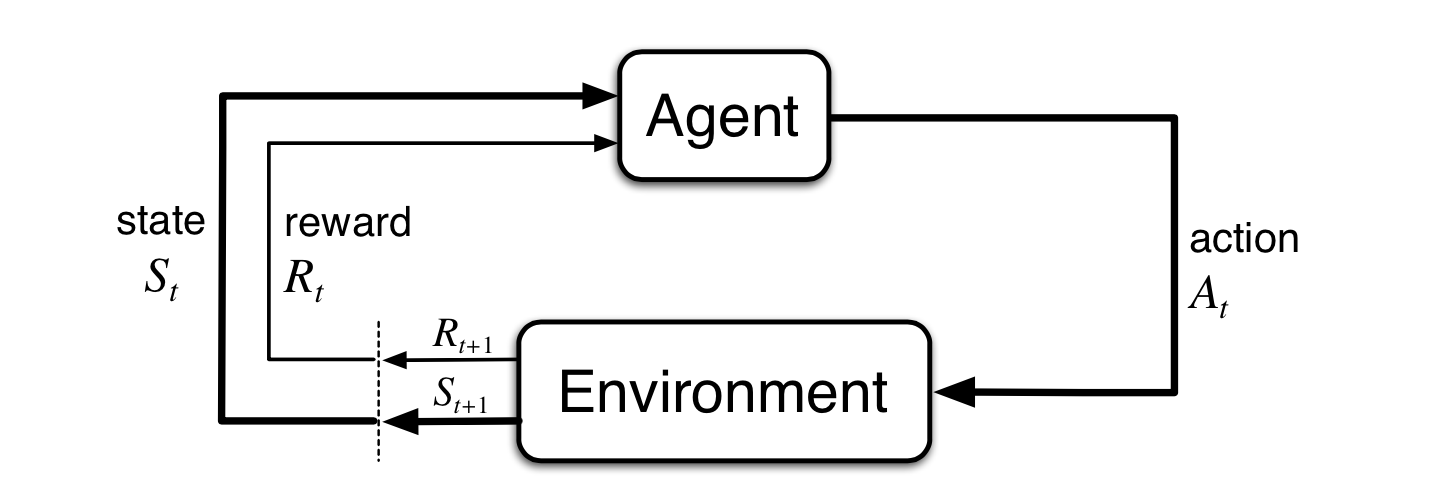
\includegraphics[width=1.25\textwidth]{img/agent_environment_untitled.png}}
  \end{center}
  \end{figure}
\end{frame}

\begin{frame}[fragile]
  \frametitle{Background}
  Belief-state MDP

\end{frame}

\begin{frame}[fragile]
  \frametitle{Background}

  Implemented MDP solvers:
  \begin{itemize}
  \item Q-learning
  \item SARSA
  \item R-MAX
  \item Thompson sampling
  \end{itemize}

  There are a lot!
  \begin{itemize}
  \item Function approximations with adaptive basis functions
  \item BOSS
  \item Spectral methods
  \item Skill chaining
  \item $\cdots$
  \end{itemize}

\end{frame}

\begin{frame}[fragile]
  \frametitle{Grocery shopping}

  the task in the POMDP framework
\end{frame}

\begin{frame}[fragile]
  \frametitle{Grocery shopping}

  how the software works, etc.
\end{frame}

\plain{demo}

\begin{frame}[fragile]
  \frametitle{Our working solver}
  \begin{itemize}
  \item Max Probability Value Iteration:
  \item Choose the most likely state from belief state to run value iteration
  \end{itemize}
\end{frame}

\begin{frame}[fragile]
  \frametitle{Our working solver}
  Value iteration:
  \begin{align*}
  v_{k+1}(s) &= \max_a \mathbb{E}[R_{t+1} + \gamma v_k(S_{t+1}) \mid S_t = s, A_t = a] \\
  &= \max_a \sum_{s'} p(s' \mid s,a) [r(s,a,s') + \gamma v_k(s')]
  \end{align*}
\end{frame}

\begin{frame}[fragile]
  \frametitle{Failed tasks}

  \begin{itemize}
  \item Value iteration as a belief-state MDP
  \item Thompson sampling
  \item ...
  \end{itemize}
\end{frame}

\plain{
  {\Large Play with it!}\\[5ex]
  
\includegraphics{img/octocat.png}\\[3ex]
  github.com/dustinvtran/bayesrl
}

\end{document}
